% !TEX encoding   = UTF8
% !TEX spellcheck = ru_RU
% !TEX root = ../seminars.tex

%%==========================================
\chapter{Основные цифровые логические схемы}
%%==========================================

\noindent
\begin{minipage}[c]{0.65\textwidth}
\parindent=2.5em

%%=====================
\section{Мультиплексор}
%%=====================
Схема с \(2^n\) входами, одним выходом и \(n\) линиями управления, которые позволяют выбрать один из входов. Мультиплексоры можно использовать для реализации булевой функции \(n\) переменных.



%%===============
\section{Декодер}
%%===============
Схема, которая получает на входе \(n\)-разрядное число и использует его для того, чтобы выбрать (то есть установить в \code{1}) одну из \(2^n\) выходных линий.

\end{minipage}\hfill\begin{minipage}{0.3\textwidth}

\vspace{-2em}
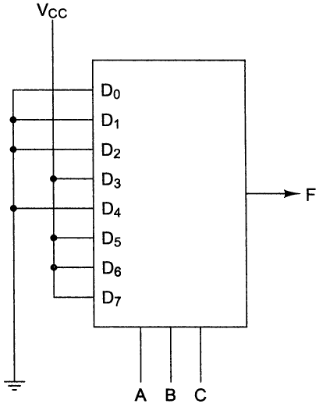
\includegraphics[width=\textwidth]{images/multiplexer.png}

\end{minipage}\medskip



%%==============================================
\section{Арифметико-логическое устройство (АЛУ)}
%%==============================================
\begin{center}
  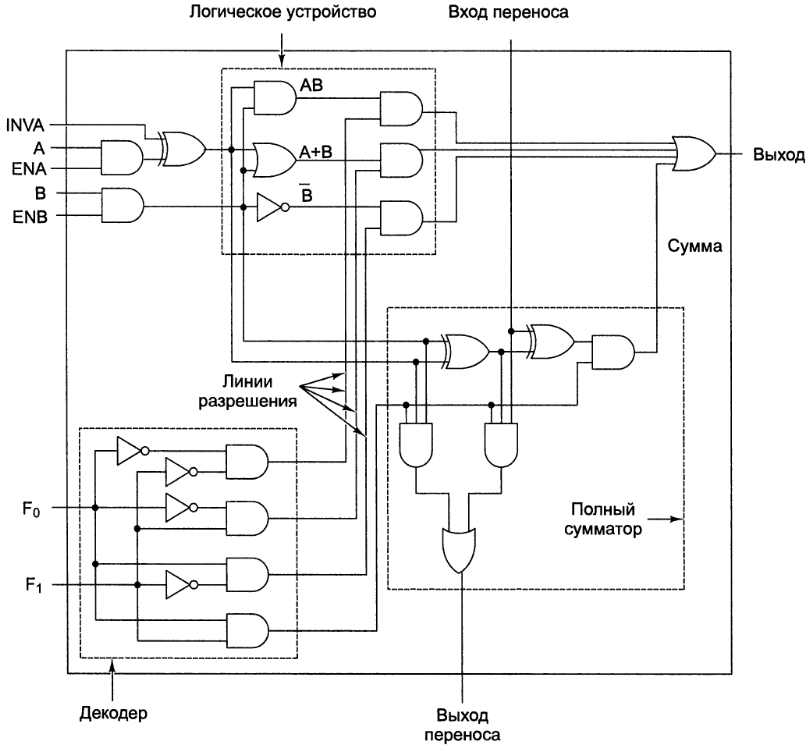
\includegraphics[width=0.8\textwidth]{images/ALU.png}
\end{center}



%%================
\section{Сумматор}
%%================
\emph{Полусумматор}~--- схема для вычисления бита суммы и бита переноса. \emph{Сумматор со сквозным переносом}.



%%==========================
\section{Тактовый генератор}
%%==========================
\noindent\begin{minipage}{0.5\columnwidth}\parindent=2.5em
  Это схема, которая вызывает серию импульсов одинаковой длительности. Интервалы между последовательными импульсами также одинаковы. Временной интервал между началом одного импульса и началом следующего называется \emph{временем такта}.
\end{minipage}\hfill\begin{minipage}{0.46\columnwidth}
  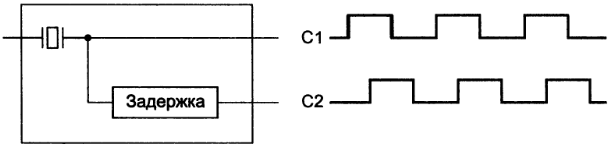
\includegraphics[width=\columnwidth]{images/clock_generator.png}
\end{minipage}

\smallskip
Частота импульсов обычно составляет от 1 до 500\,МГц (время такта от 1000 до 2\,нс). Частота тактового генератора как правило контролируется кварцевым генератором, позволяющим добиться высокой точности. Схемы могут запускаться не только уровнем сигнала, но также фронтом или спадом.



%%=======================
\section{Элементы памяти}
%%=======================
\begin{flushleft}\begin{minipage}[c]{0.3\columnwidth}\newcommand{\vsp}{\vspace{0.5cm}}
    SR-защёлка
    \par\vsp синхронная SR-защёлка
    \par\vsp триггер
    \par\vsp D-триггер
  \end{minipage}\hfill\begin{minipage}[c]{0.65\columnwidth}
    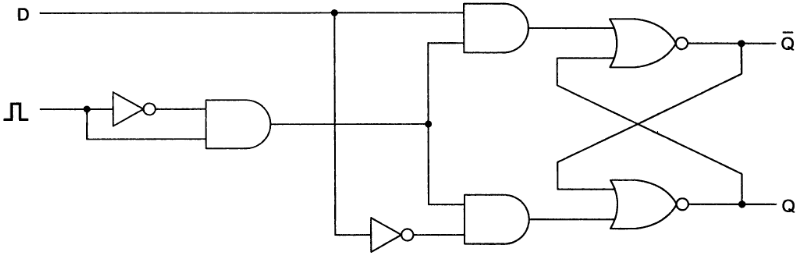
\includegraphics[width=\columnwidth]{images/D-trigger.png}
\end{minipage}\end{flushleft}



%%================
\WhatToReadSection
%%================
\begin{tabular}{@{}l@{}}
  \citeauthor[глава~2, стр.~144--200, 220--248; глава~5, стр.~601--638]{Harris:2015:ru} \\
  \citeauthor[глава~3, стр.~182--208]{Tanenbaum:2013:ru}
\end{tabular}



%%===============
\ExercisesSection
%%===============
\begin{exercise}
\item Постройте двухразрядный \emph{компаратор}, то есть схему, которая получает на вход два двухбитовых слова и выдаёт на выход \code{1}, если слова равны, и \code{0}, если они не равны.

\item \emph{Схема сдвига} имеет \(2^n\) входных битов. Выходные данные~--- это входные данные, сдвинутые на один бит. Линия управления определяет направление сдвига: \code{0}~--- влево, \code{1}~--- вправо. Постройте схему сдвига для четырёхразрядного слова.

\item Нарисуйте логическую схему двухразрядного \emph{кодера}, который содержит 4 входные и 2 выходные линии. Одна из входных линий всегда равна~\code{1}. Двухразрядное двоичное число на двух выходных линиях показывает, какая именно входная линия равна~\code{1}.

\item Нарисуйте логическую схему двухразрядного \emph{демультиплексора}, у которого сигнал на единственной входной линии направляется к одной из четырёх выходных линий в зависимости от значений двух линий управления.

\end{exercise}
